\documentclass[12pt, letterpaper]{article}
\usepackage[T1]{fontenc}
\usepackage[utf8]{inputenc}
\usepackage{graphicx}
\usepackage{caption}
\usepackage{subcaption}
\usepackage{geometry}
\usepackage{float}
\usepackage{amsmath}
\usepackage{fancyhdr}
\usepackage{pdfpages}

% Page Geometry
\geometry{margin=1in}
\setlength{\headheight}{14.49998pt}
\addtolength{\topmargin}{-2.49998pt}

\graphicspath{{./Pictures/}}
\pdfcompresslevel=9
\pdfobjcompresslevel=3
\pdfminorversion=5

% Header/Footer Setup
\pagestyle{fancy}
\lhead{EEE3307: Lab 4 Report}
\rhead{Yousef Awad}
\cfoot{\thepage}

\title{
    \vspace{1in}
    \textbf{\huge EEE3307 Electronics I} \\[0.5em]
    \textbf{\Large Experiment \#4: Transistor AC Amplifiers}
    \vspace{1.5in}
}
\author{
    \textbf{Name:} Yousef Alaa Awad \\
    \textbf{Partners:} Egor Shevchenko and Abram Tadros
}
\date{Lab Session: March 26, 2026}

\begin{document}

\maketitle
\newpage

%----------------------------------------------------------------------------------------
%	1. INTRODUCTION
%----------------------------------------------------------------------------------------
\section{Introduction}
The objective of this experiment was to study the performance of common-emitter (CE) transistor AC amplifiers. Specifically, the experiment focused on the impact of the emitter bypass capacitor ($C_E$) on voltage gain and the optimization of the DC operating point (Q-point) to maximize the symmetrical unclipped AC output swing. By placing the Q-point at the center of the AC load line, the amplifier can provide the largest possible signal replica before clipping occurs due to saturation or cutoff.

%----------------------------------------------------------------------------------------
%	2. EXPERIMENTAL PROCEDURE
%----------------------------------------------------------------------------------------
\section{Experimental Procedure}
The experiment followed the steps outlined in the Lab Manual for Experiment \#4:
\begin{enumerate}
	\item \textbf{Initial Biasing:} A CE amplifier was constructed using $V_{CC}=12V, R_C=6.2k\Omega, R_E=1.8k\Omega, R_L=2.2k\Omega$. $R_1$ and $R_2$ were chosen based on pre-lab calculations ($R_1 \approx 164k\Omega, R_2 \approx 33k\Omega$) to establish $I_{CQ} \approx 1mA$.
	\item \textbf{Maximum Unclipped Output (with $C_E$):} A 5 kHz sinusoidal signal was applied, and the input amplitude was increased until the output waveform began to clip. The maximum unclipped output was recorded.
	\item \textbf{Effect of $C_E$ Removal:} The bypass capacitor $C_E$ was removed, and the maximum unclipped output was re-measured to observe the drastic reduction in gain caused by emitter degeneration.
	\item \textbf{Optimized Biasing:} $R_1$ and $R_2$ were replaced with values calculated to center the Q-point on the AC load line ($R_1 = 100k\Omega, R_2 = 34k\Omega$). The maximum unclipped output was measured again.
	\item \textbf{Optimized Biasing without $C_E$:} Step 4 was repeated with $C_E$ removed.
	\item \textbf{Impact of $R_C$ Variation:} $R_C$ was changed to $3.2k\Omega$, and the resulting $I_{CQ}$ was measured to verify bias stability.
\end{enumerate}

\pagebreak
%----------------------------------------------------------------------------------------
%	3. COMPUTER SIMULATION
%----------------------------------------------------------------------------------------
\section{Computer Simulation}
Prior to laboratory implementation, the circuits were simulated to verify theoretical performance and determine the expected Q-points and unclipped output swings.

\subsection{Initial Bias Configuration (Parts 1 \& 2)}
The initial circuit schematic and the resulting DC operating point data are shown below. The simulation confirmed $I_{CQ} \approx 1 mA$ and provided the baseline for maximum unclipped output with the bypass capacitor $C_E$ included.

\begin{figure}[H]
    \centering
    \begin{subfigure}[b]{0.48\textwidth}
        \centering
        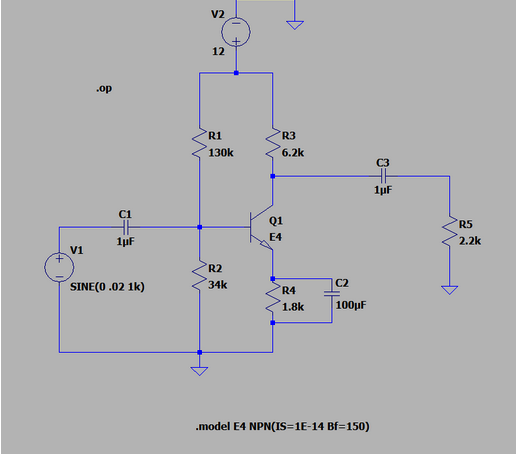
\includegraphics[width=\textwidth]{simulation_part1and2_schematic.png}
        \caption{Simulation Schematic}
    \end{subfigure}
    \hfill
    \begin{subfigure}[b]{0.48\textwidth}
        \centering
        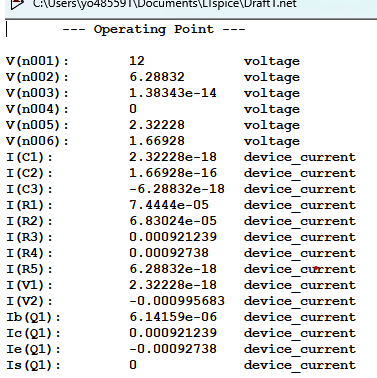
\includegraphics[width=\textwidth]{simulation_part1and2_numbers.png}
        \caption{Operating Point Data}
    \end{subfigure}
    \caption{Simulation setup for initial biasing ($R_1 \approx 164k\Omega, R_2 \approx 33k\Omega$).}
\end{figure}

\begin{figure}[H]
    \centering
    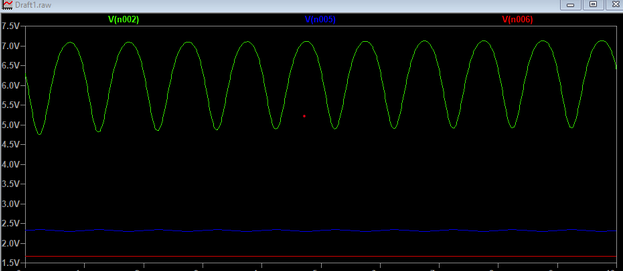
\includegraphics[width=0.7\textwidth]{simulation_part1and2_waveform.png}
    \caption{Simulation waveform showing unclipped output for the initial configuration.}
\end{figure}

\subsection{Optimized Bias Configuration (Parts 3-6)}
The schematic was modified to center the Q-point on the AC load line. The simulation below shows the improved output swing capability and the effects of varying $R_C$ and $C_E$.

\begin{figure}[H]
    \centering
    \begin{subfigure}[b]{0.55\textwidth}
        \centering
        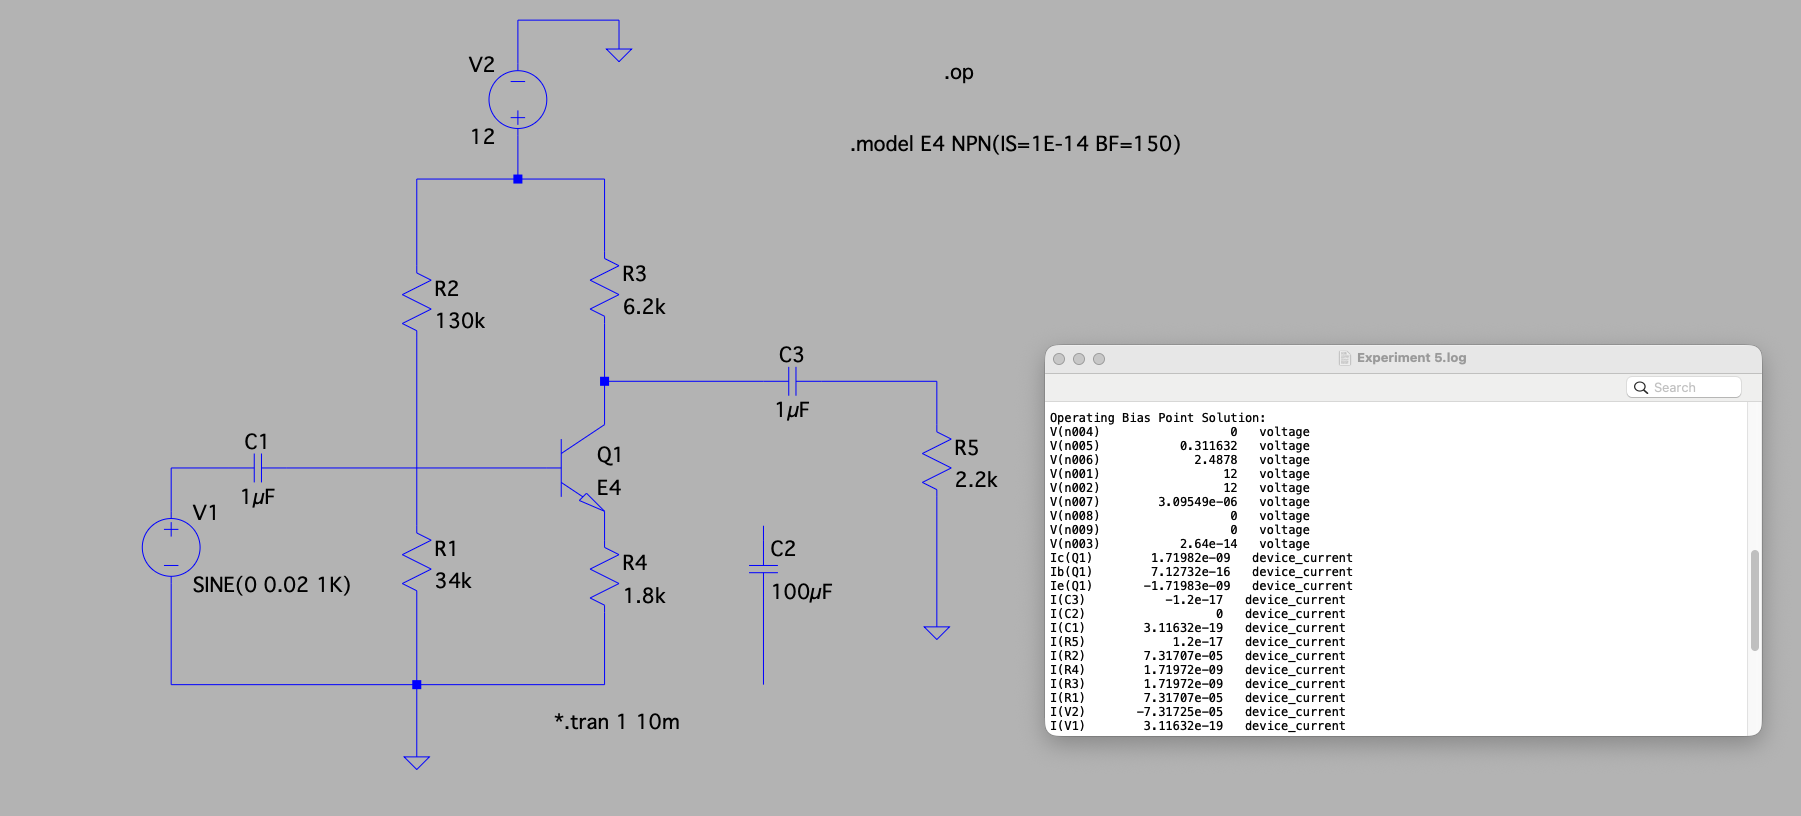
\includegraphics[width=\textwidth]{simulation_part3and4and5and6_schematic.png}
        \caption{Optimized Schematic}
    \end{subfigure}
    \hfill
    \begin{subfigure}[b]{0.42\textwidth}
        \centering
        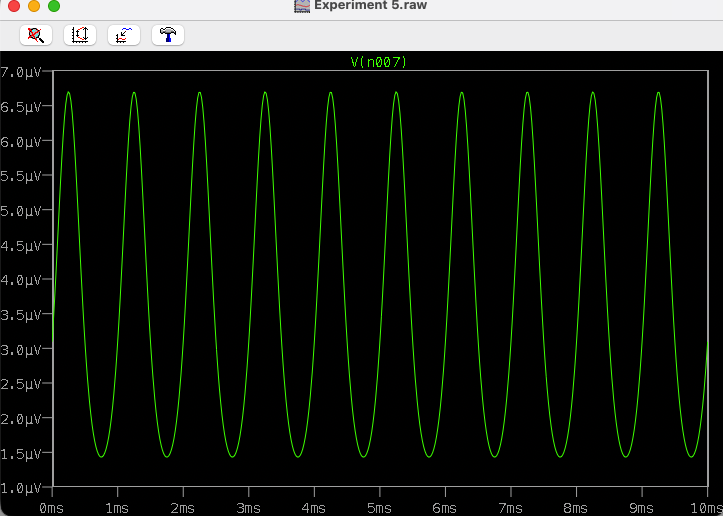
\includegraphics[width=\textwidth]{simulation_part3and4and5and6_waveform.png}
        \caption{Optimized Waveform}
    \end{subfigure}
    \caption{Simulation results for the optimized bias configuration.}
\end{figure}

\pagebreak
%----------------------------------------------------------------------------------------
%	4. RESULTS AND DISCUSSION
%----------------------------------------------------------------------------------------
\section{Results and Discussion}

\subsection{Initial Circuit Performance (Parts 1 \& 2)}
The initial circuit was built as shown in the breadboard photo (Figure \ref{fig:part1_bb}). The measured quiescent current $I_{CQ}$ was $0.9997 mA$, which is nearly identical to the design target of $1mA$ (Figure \ref{fig:part1_icq}) and the simulation results.

\begin{figure}[H]
	\centering
	\begin{subfigure}[b]{0.45\textwidth}
		\centering
		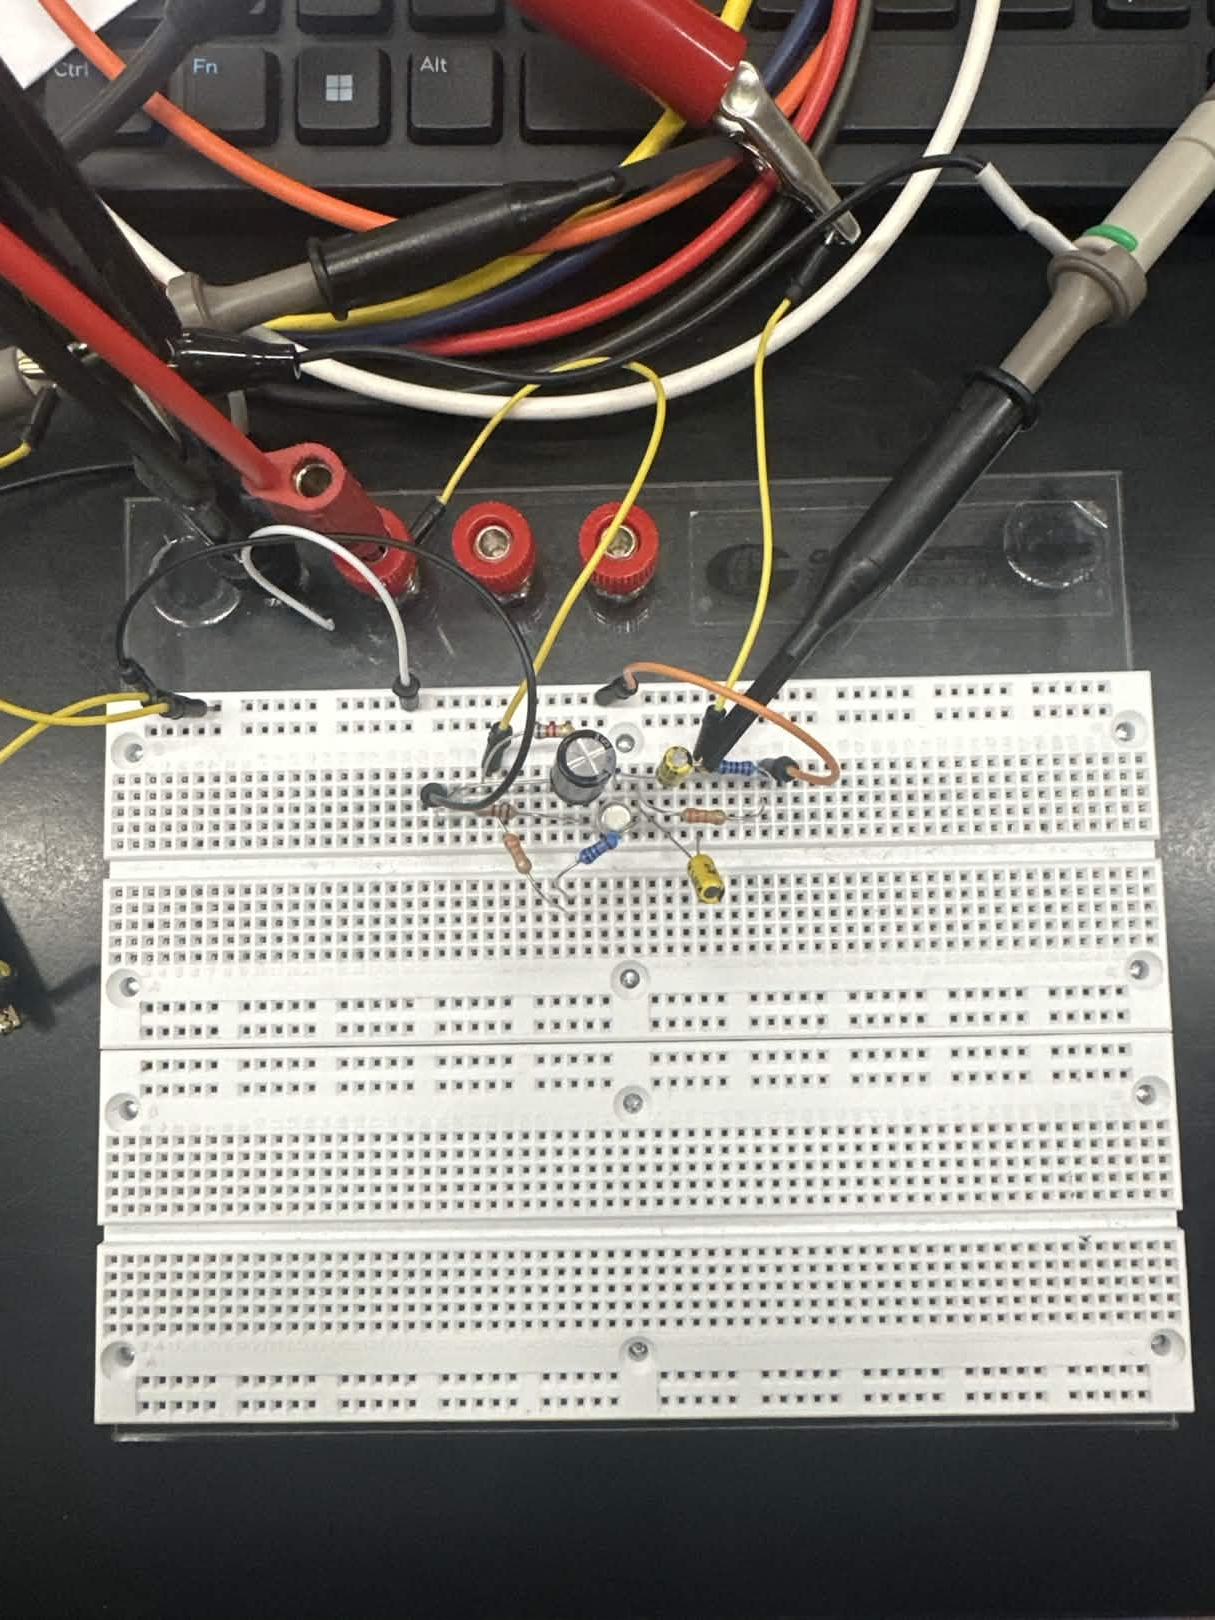
\includegraphics[width=\textwidth]{part1_breadboard.jpg}
		\caption{Breadboard assembly for Part 1.}
		\label{fig:part1_bb}
	\end{subfigure}
	\hfill
	\begin{subfigure}[b]{0.45\textwidth}
		\centering
		\includegraphics[width=\textwidth]{part1_icq.jpg}
		\caption{Measured $I_{CQ} \approx 1 mA$.}
		\label{fig:part1_icq}
	\end{subfigure}
	\caption{Initial biasing measurements.}
\end{figure}

With the bypass capacitor $C_E$ included, the amplifier exhibited high gain. The maximum unclipped output waveform is shown in Figure \ref{fig:part2_scope}, where the green trace (Vout) shows significant amplification of the yellow trace (Vin).

\begin{figure}[H]
	\centering
	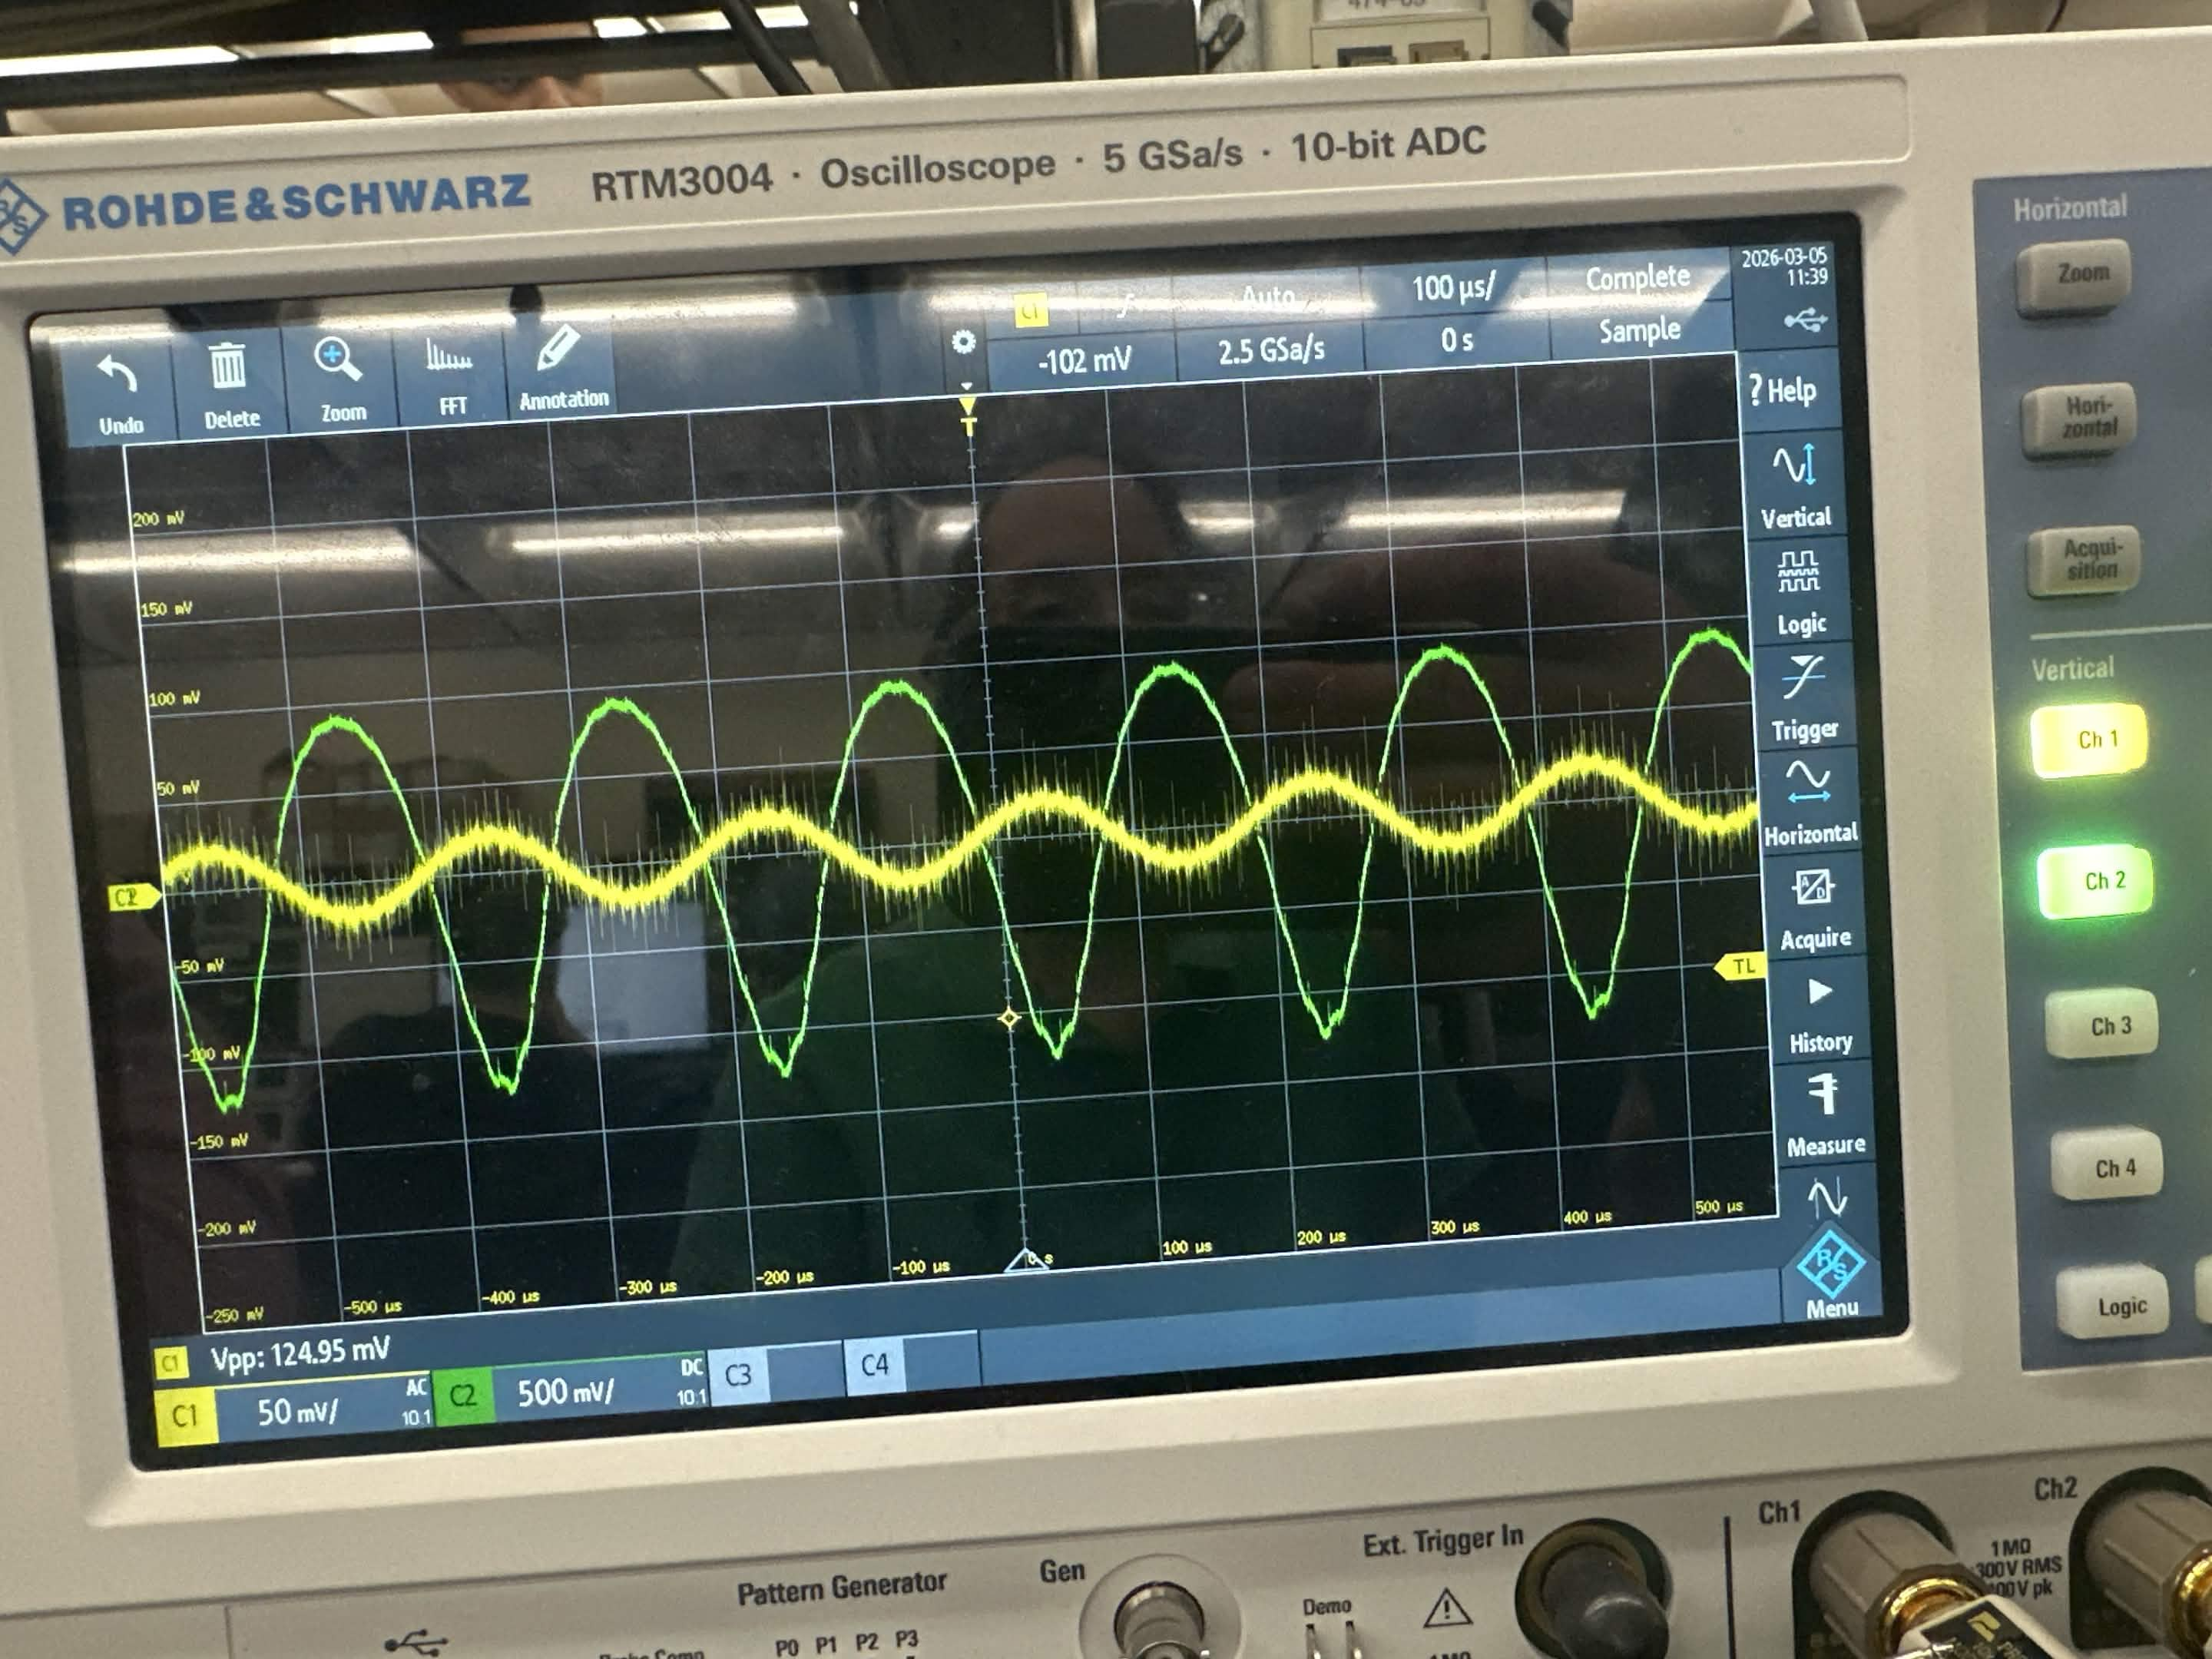
\includegraphics[width=0.6\textwidth]{part2_yellowVin_greenVout.jpg}
	\caption{Oscilloscope trace for Part 2 (with $C_E$).}
	\label{fig:part2_scope}
\end{figure}

\subsection{Effect of Emitter Degeneration (Part 3)}
Removing $C_E$ introduces negative feedback through $R_E$. As seen in Figure \ref{fig:part3_scope}, the gain dropped significantly, and the maximum unclipped output was reduced because the signal swing is now limited by the degeneration.

\begin{figure}[H]
	\centering
	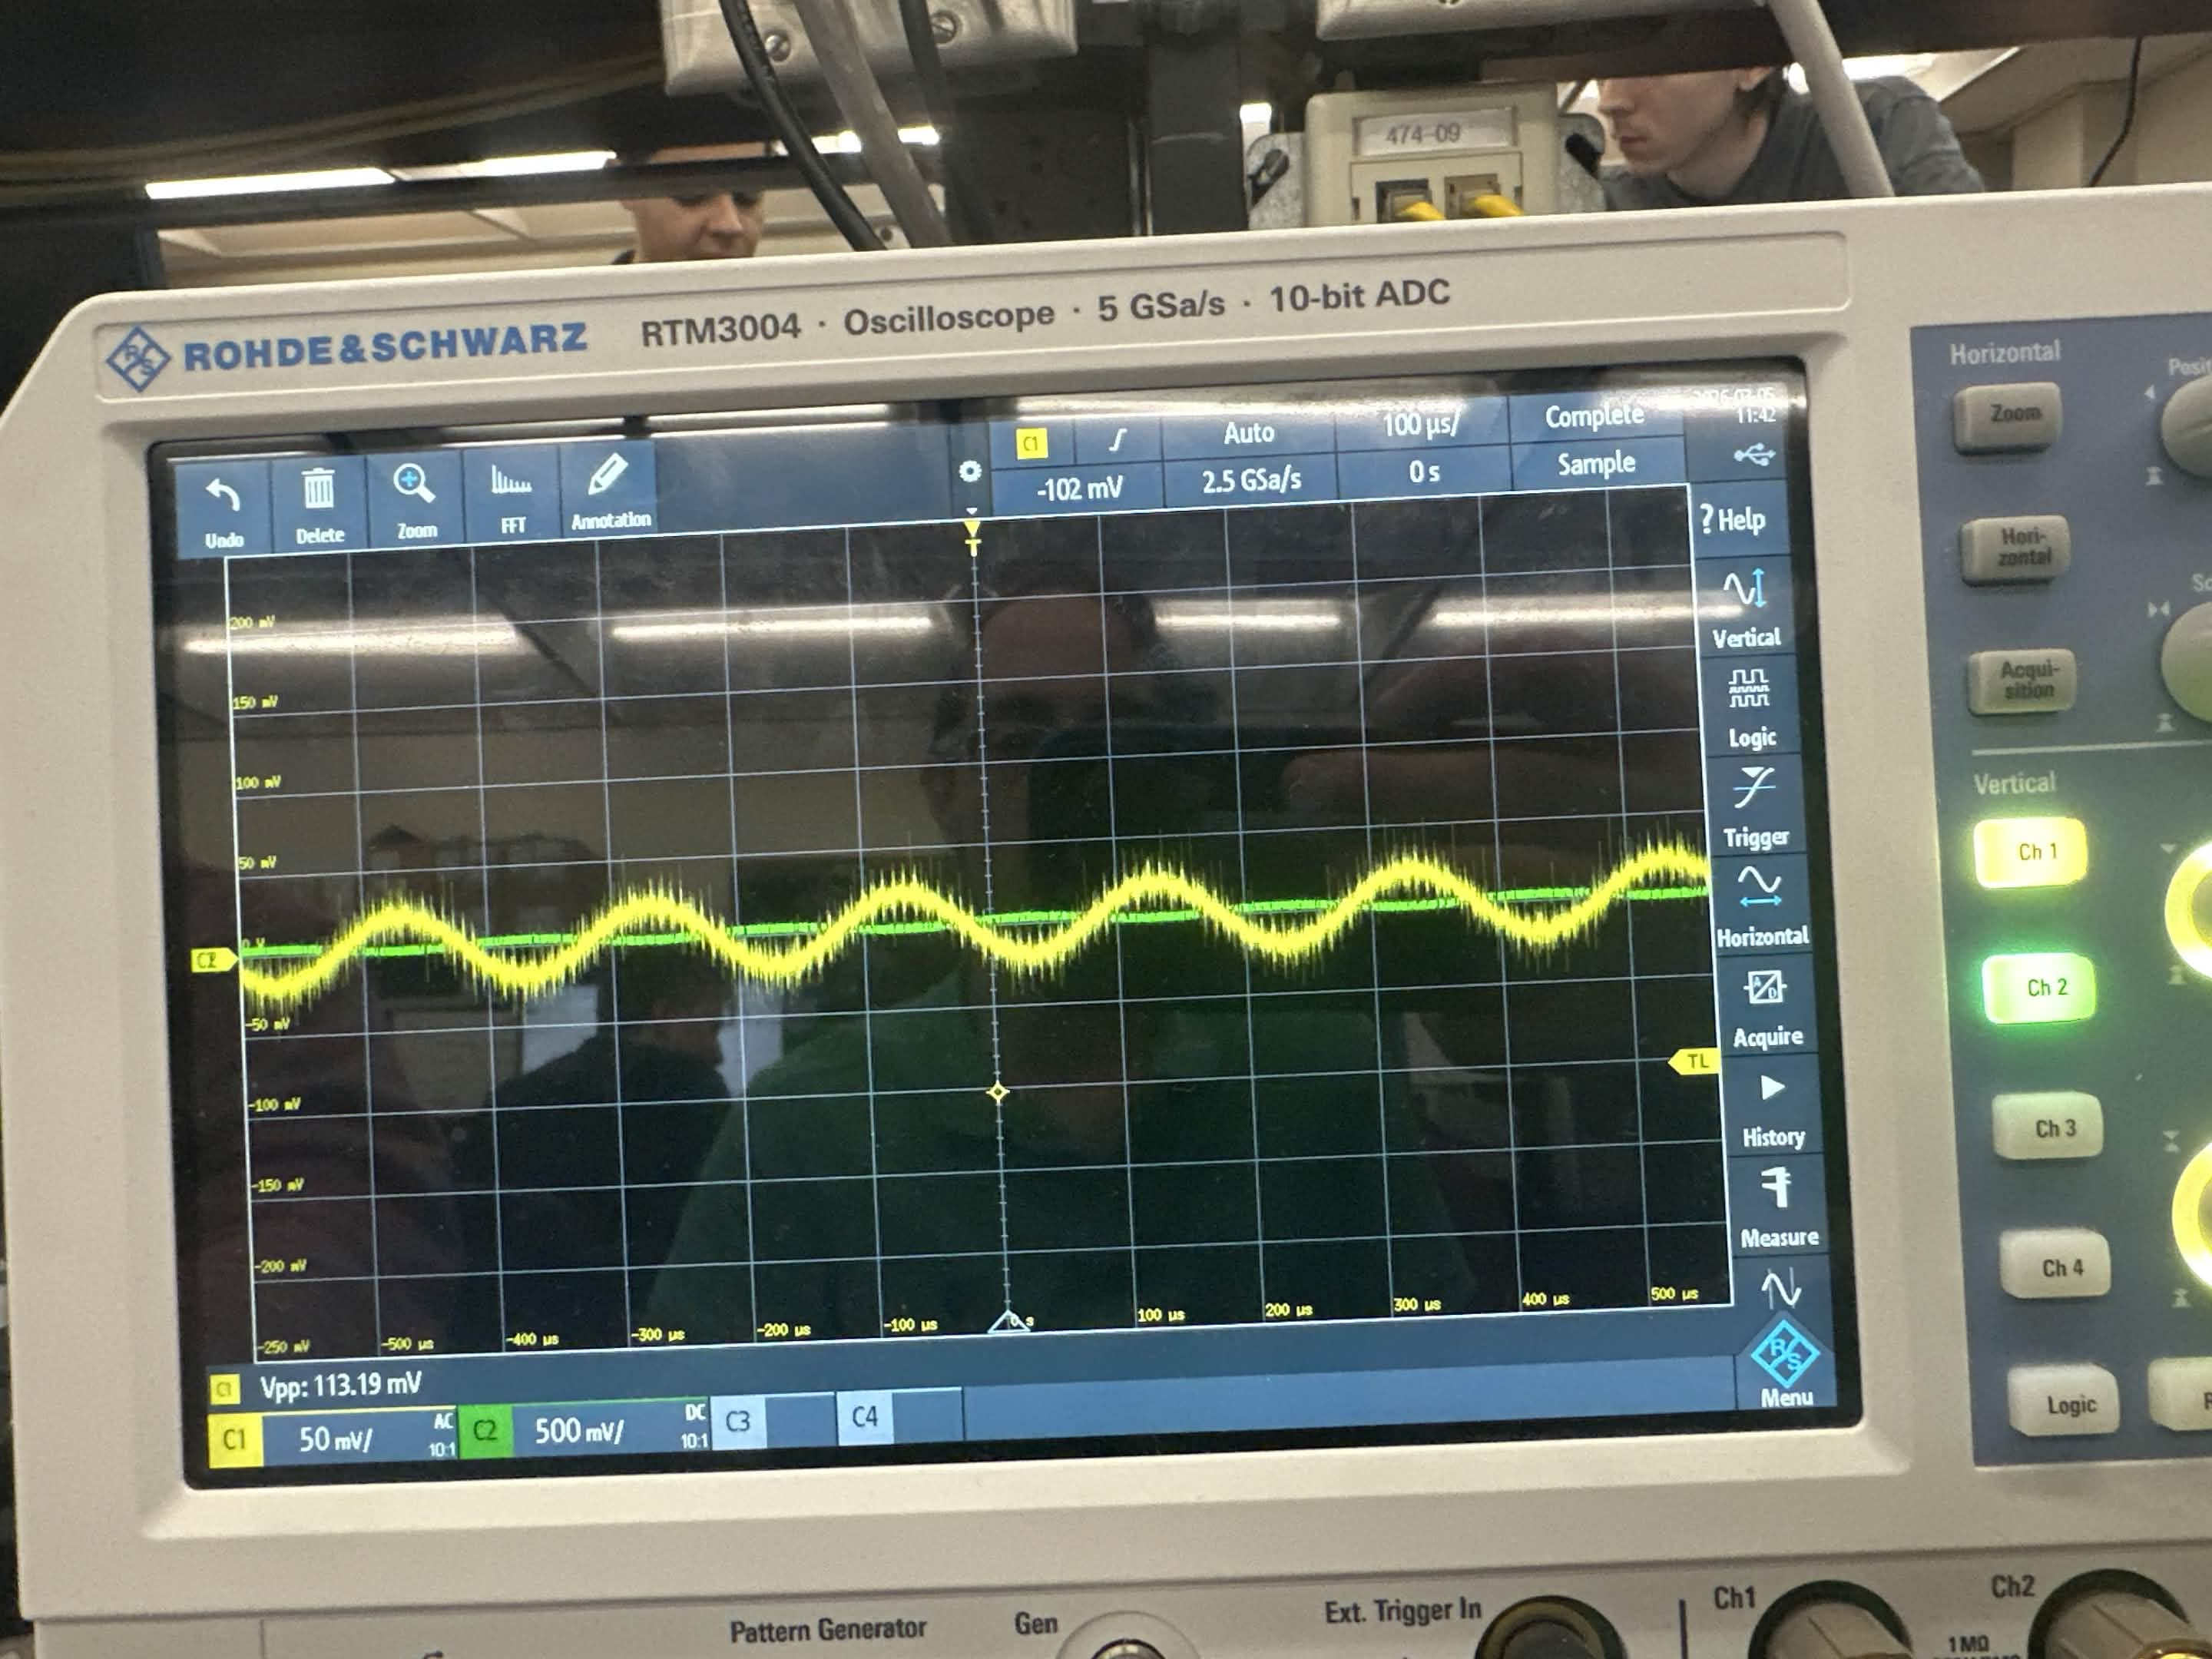
\includegraphics[width=0.6\textwidth]{part3_CeRemoved_yellowVin_greenVout.jpg}
	\caption{Oscilloscope trace for Part 3 ($C_E$ removed).}
	\label{fig:part3_scope}
\end{figure}

\pagebreak
\subsection{Optimized Q-Point Performance (Parts 4 \& 5)}
To maximize the output swing, the Q-point was shifted by changing $R_1$ to $100k\Omega$ and $R_2$ to $34k\Omega$. This adjustment centers the Q-point on the AC load line. Figure \ref{fig:part4_scope} shows the resulting waveforms. The output swing is visibly larger and more symmetrical than in the previous configuration. Removing $C_E$ again reduced the gain as expected (Figure \ref{fig:part5_scope}).

\begin{figure}[H]
	\centering
	\begin{subfigure}[b]{0.48\textwidth}
		\centering
		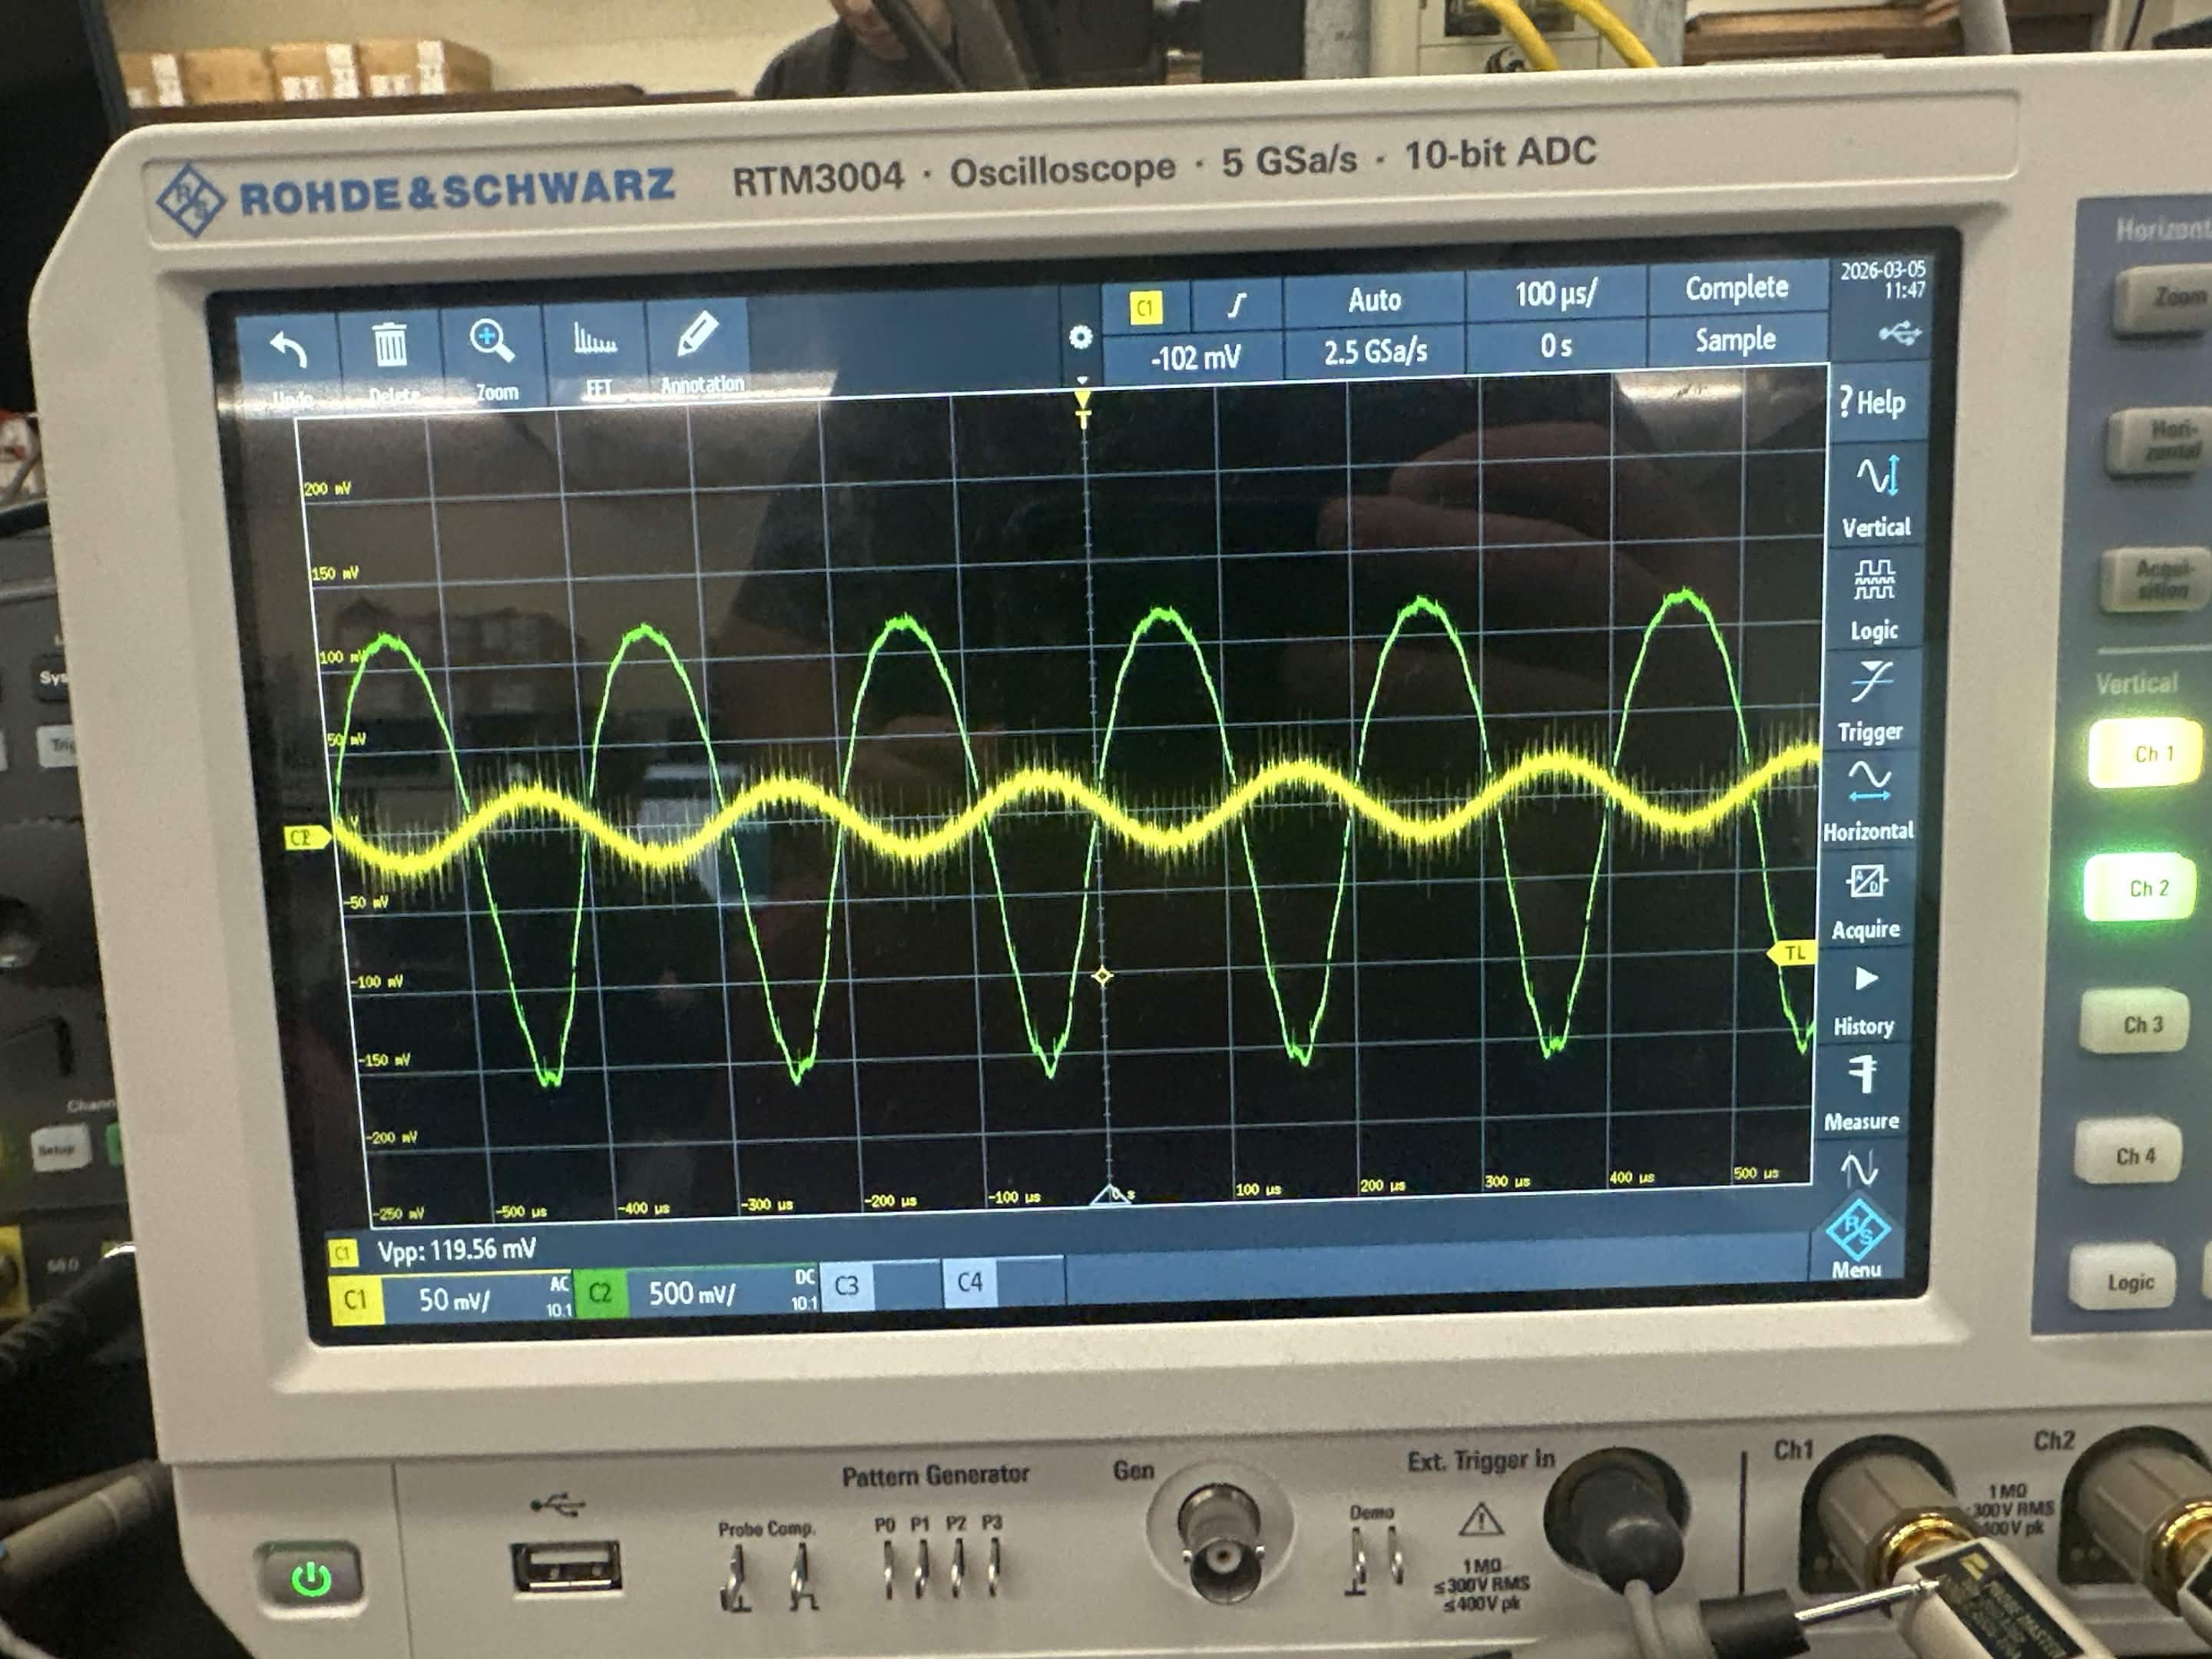
\includegraphics[width=\textwidth]{part4_r1_100k_r2_34k_yellowVin_greenVout.jpg}
		\caption{Part 4: Optimized bias with $C_E$.}
		\label{fig:part4_scope}
	\end{subfigure}
	\hfill
	\begin{subfigure}[b]{0.48\textwidth}
		\centering
		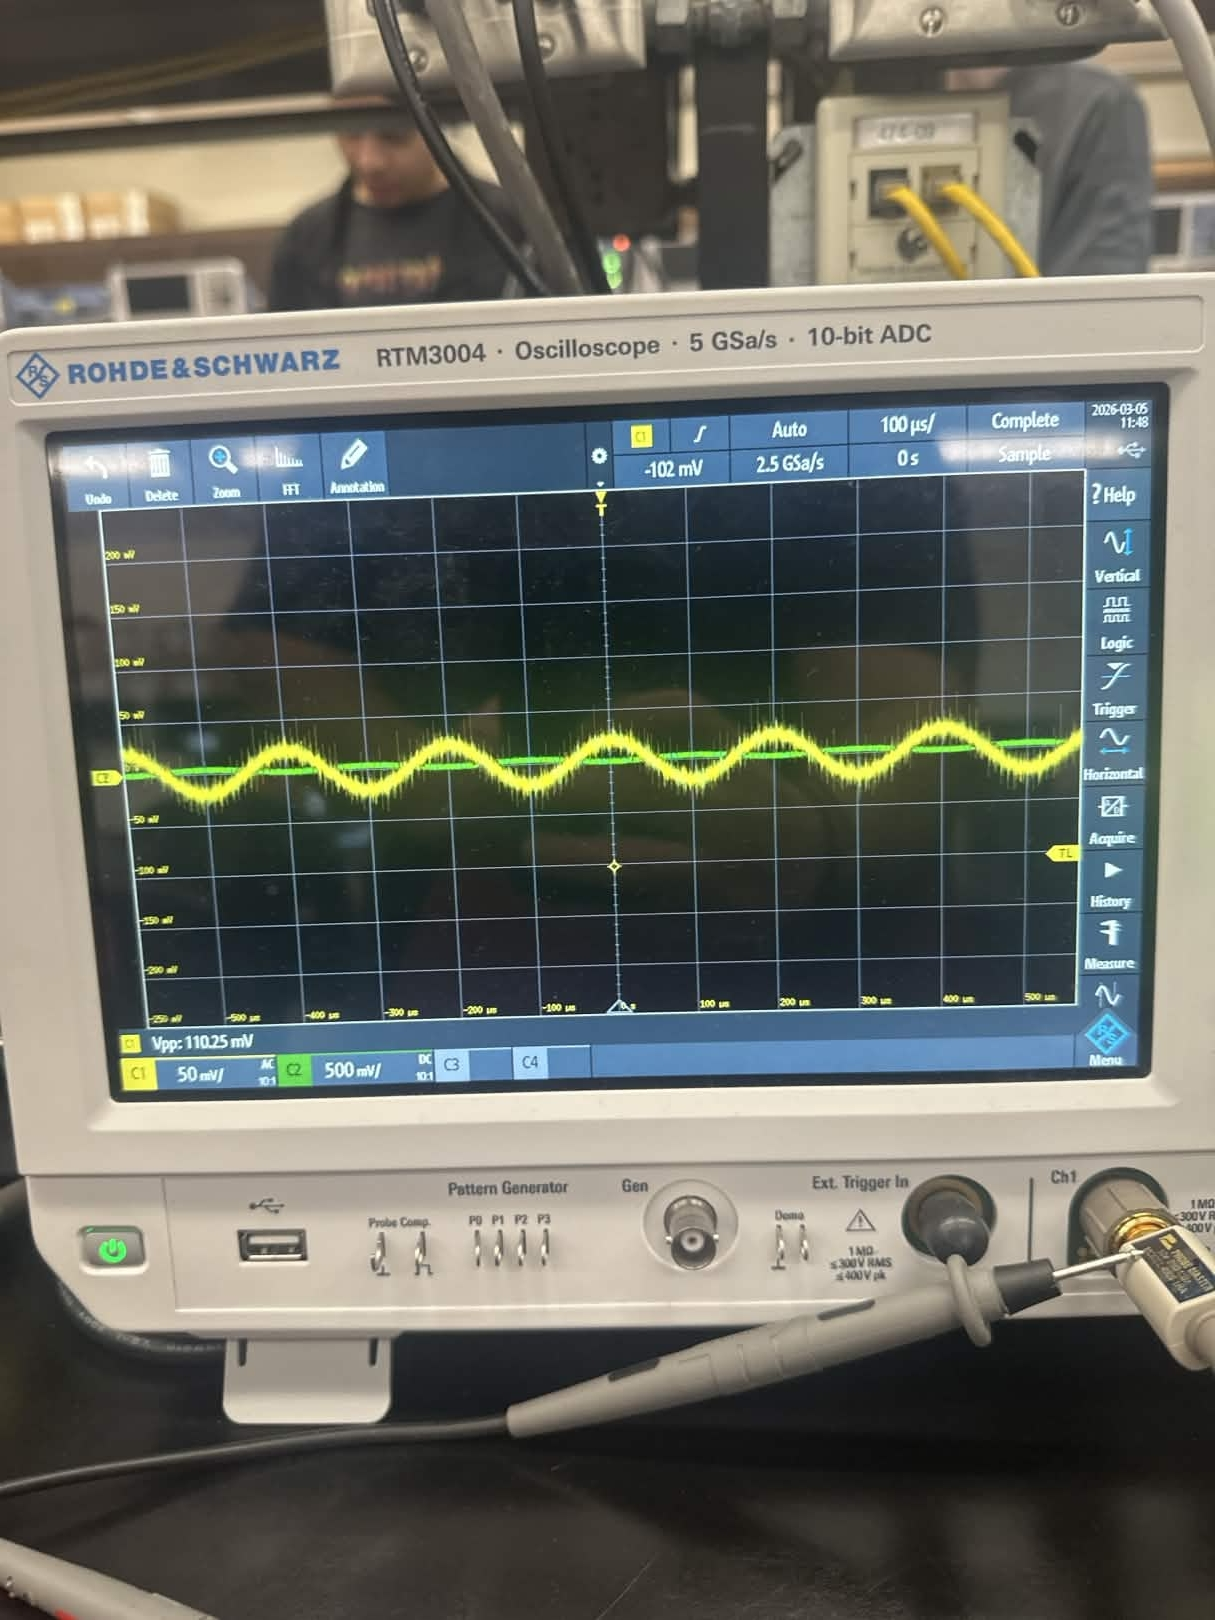
\includegraphics[width=\textwidth]{part5_r1_100k_r2_34k_yellowVin_greenVout.jpg}
		\caption{Part 5: Optimized bias without $C_E$.}
		\label{fig:part5_scope}
	\end{subfigure}
	\caption{Amplifier performance with optimized biasing.}
\end{figure}

\subsection{Bias Stability and $R_C$ Variation (Part 6)}
Changing $R_C$ to $3.2k\Omega$ did not significantly affect the collector current. The measured $I_{CQ}$ remained at $1.0028 mA$ (Figure \ref{fig:part6_icq}). This confirms that the voltage-divider bias circuit with an emitter resistor provides excellent DC stability, as $I_{CQ}$ is primarily determined by the base-side Thevenin voltage and $R_E$, rather than the collector load resistance $R_C$.

\begin{figure}[H]
	\centering
	\includegraphics[width=0.5\textwidth]{part6_icq.jpg}
	\caption{Measured $I_{CQ}$ with $R_C = 3.2k\Omega$.}
	\label{fig:part6_icq}
\end{figure}

\clearpage
%----------------------------------------------------------------------------------------
%	4. PRE-LABORATORY CALCULATIONS
%----------------------------------------------------------------------------------------
\section{Pre-Laboratory Calculations}
The hand-calculated pre-laboratory derivations are attached below. They match the experimental results and the simulation waveforms obtained during the preparation phase.
\pagebreak
\includepdf[pages=-]{prelab.pdf}

%----------------------------------------------------------------------------------------
%	5. CONCLUSION
%----------------------------------------------------------------------------------------
\section{Conclusion}
This experiment validated the theory of common-emitter transistor AC amplifiers. We demonstrated that the bypass capacitor $C_E$ is critical for achieving high voltage gain, while its removal improves stability at the cost of gain. Furthermore, we verified that optimizing the Q-point at the center of the AC load line significantly increases the maximum unclipped output voltage. Finally, the stability of the voltage-divider bias was confirmed by observing that the collector current $I_{CQ}$ remains constant despite changes in the collector resistance $R_C$.
\end{document}
